%% This is file `elsarticle-template-1-num.tex',
%%
%% Copyright 2009 Elsevier Ltd
%%
%% This file is part of the 'Elsarticle Bundle'.
%% ---------------------------------------------
%%
%% It may be distributed under the conditions of the LaTeX Project Public
%% License, either version 1.2 of this license or (at your option) any
%% later version.  The latest version of this license is in
%%    http://www.latex-project.org/lppl.txt
%% and version 1.2 or later is part of all distributions of LaTeX
%% version 1999/12/01 or later.
%%
%% Template article for Elsevier's document class `elsarticle'
%% with numbered style bibliographic references
%%
%% $Id: elsarticle-template-1-num.tex 149 2009-10-08 05:01:15Z rishi $
%% $URL: http://lenova.river-valley.com/svn/elsbst/trunk/elsarticle-template-1-num.tex $
%%
\documentclass[preprint,12pt]{elsarticle}

%% Use the option review to obtain double line spacing
%% \documentclass[preprint,review,12pt]{elsarticle}

%% Use the options 1p,twocolumn; 3p; 3p,twocolumn; 5p; or 5p,twocolumn
%% for a journal layout:
%% \documentclass[final,1p,times]{elsarticle}
%% \documentclass[final,1p,times,twocolumn]{elsarticle}
%% \documentclass[final,3p,times]{elsarticle}
%% \documentclass[final,3p,times,twocolumn]{elsarticle}
%% \documentclass[final,5p,times]{elsarticle}
%% \documentclass[final,5p,times,twocolumn]{elsarticle}

%% The graphicx package provides the includegraphics command.
\usepackage{graphicx}
%% The amssymb package provides various useful mathematical symbols
\usepackage{amssymb}
%% The amsthm package provides extended theorem environments
%% \usepackage{amsthm}

%% The lineno packages adds line numbers. Start line numbering with
%% \begin{linenumbers}, end it with \end{linenumbers}. Or switch it on
%% for the whole article with \linenumbers after \end{frontmatter}.
\usepackage{lineno}


%% natbib.sty is loaded by default. However, natbib options can be
%% provided with \biboptions{...} command. Following options are
%% valid:

%%   round  -  round parentheses are used (default)
%%   square -  square brackets are used   [option]
%%   curly  -  curly braces are used      {option}
%%   angle  -  angle brackets are used    <option>
%%   semicolon  -  multiple citations separated by semi-colon
%%   colon  - same as semicolon, an earlier confusion
%%   comma  -  separated by comma
%%   numbers-  selects numerical citations
%%   super  -  numerical citations as superscripts
%%   sort   -  sorts multiple citations according to order in ref. list
%%   sort&compress   -  like sort, but also compresses numerical citations
%%   compress - compresses without sorting
%%
%% \biboptions{comma,round}

% \biboptions{}

\journal{Journal Name}

\usepackage[top=1in, bottom=1.5in, left=1in, right=1in]{geometry}
\usepackage[
    %backend=biber, 
    natbib=true,
    style=numeric,
    sorting=none
]{biblatex}
\addbibresource{sample.bib}

\begin{document}


%\begin{frontmatter}

%% Title, authors and addresses

%\title{b~flavored Jets as a Handle for Direct Measurement of ggH production of the Higgs and its subsequent decay to $b\bar{b}$ during Run 3 and Run 4 at the LHC/HL-LHC}

%% use the tnoteref command within \title for footnotes;
%% use the tnotetext command for the associated footnote;
%% use the fnref command within \auth or or \address for footnotes;
%% use the fntext command for the associated footnote;
%% use the corref command within \author for corresponding author footnotes;
%% use the cortext command for the associated footnote;
%% use the ead command for the email address,
%% and the form \ead[url] for the home page:
%%
%% \title{Title\tnoteref{label1}}
%% \tnotetext[label1]{}
 %\author{Prof. Isobel Ojalvo}
 %\ead{iojalvo@princeton.edu}
%% \ead[url]{home page}
%% \fntext[label2]{}
%% \cortext[cor1]{}
%% \address{Address\fnref{label3}}
%% \fntext[label3]{}


%% use optional labels to link authors explicitly to addresses:
%% \author[label1,label2]{<author name>}
%% \address[label1]{<address>}
%% \address[label2]{<address>}

%\author{John Smith}

%\address{California, United States}

%\begin{abstract}
%% Text of abstract
%Suspendisse potenti. Suspendisse quis sem elit, et mattis nisl. Phasellus consequat erat eu velit rhoncus non pharetra neque auctor. Phasellus eu lacus quam. Ut ipsum dolor, euismod aliquam congue sed, lobortis et orci. Mauris eget velit id arcu ultricies auctor in eget dolor. Pellentesque suscipit adipiscing sem, imperdiet laoreet dolor elementum ut. Mauris condimentum est sed velit lacinia placerat. Vestibulum ante ipsum primis in faucibus orci luctus et ultrices posuere cubilia Curae; Nullam diam metus, pharetra vitae euismod sed, placerat ultrices eros. Aliquam tincidunt dapibus venenatis. In interdum tellus nec justo accumsan aliquam. Nulla sit amet massa augue.
%\end{abstract}


%\begin{keyword}
%Science \sep Publication \sep Complicated
%% keywords here, in the form: keyword \sep keyword

%% MSC codes here, in the form: \MSC code \sep code
%% or \MSC[2008] code \sep code (2000 is the default)

%\end{keyword}

%\end{frontmatter}

%%
%% Start line numbering here if you want
%%
%\linenumbers

%% main text


\noindent
\textbf{Precision Measurements of the Higgs in its Decay to Taus}

\section{Overview}
As a member of the Compact Muon Solenoid (CMS) experiment~\cite{CMS-JINST} at the LHC, 
I propose to introduce novel methods to the current and future online CMS trigger systems 
in order to improve the identification and acquisition of events containing rare particle
physics phenomena. 
With the arrival of new high-level synthesis technologies that allow us
to quickly and easily translate advanced algorithms into hardware 
description language, it is possible to target specific Standard Model Higgs
production mechanisms at the event level. We are developing topological triggers 
to identify events that contain two back-to-back jets, indicative of 
Vector Boson Fusion, a single fat jet with sub-structure, indicative of a boosted
object topology or a long lived particle (LLP) with calorimeter deposits that are
displaced in time. %Or a an anomaly based trigger... finish me.

Currently I am leading the CMS physics analysis in the characterization of the Higgs 
Boson in its decay to tau ($\tau$) leptons with the full Run 2 dataset; previously as 
a postdoc I led the analysis effort which resulted in the first observation of the 
Higgs in its decay to $\taus$'s by a single experiment~\cite{HIG16043}. 
This observation was the 
result of iterative development and improvements to the $\tau$ trigger, reconstruction 
and identification by the CMS collaboration. I have contributed to these efforts and served 
in leadership positions in the CMS collaboration first as the developer of the Level-1 (L1)
trigger $\tau$ algorithm, put into place in 2015, then as the convener of the tau trigger
development group (2014-2015) and later as the convener of the tau physics object group 
(2015-2018). Currently, I serve as the US CMS L1 Trigger Operations deputy. 
As a new faculty member at Princeton, I have used my startup funding to hire an 
engineer, Luis Perez Moreno, who is working on CMS L1 Trigger firmware development
for Run 3 and Run 4 with the US APD hardware consortium. He is supporting operations 
of the calorimeter trigger at 
CMS and will work with postdoc, Pallabi Das, and graduate student, Stephanie Kwan, on
implementation. Based upon our first developments of
this project, Stephanie Kwan, has received the NSF graduate student research award
and her tuition and salary is supported by the NSF. She and Pallabi Das are stationed
at CERN, supporting CMS Level-1 trigger operations, their cost of living is supported 
through detector operations.

My group's primary physics activities are the precision measurements of the electroweak symmetry breaking mechanism, 
precision measurements of the the Higgs Yukawa coupling and searches for associated new physics phenomena. 
The observation of the Higgs in its decay to $\tau$'s by the CMS experiment in 2017 sets the context for my 
current and future research program. It strengthens the case for using the Higgs in its decay to $\tau$'s for 
detailed study of the properties of this new boson. 
This physics process will also be leveraged in searches for beyond the standard model supersymmetric Higgs bosons. 

%\section{Proposed Research Direction}

The basic framework of the Standard Model (SM) works for many particle physics interactions and measurements but is not an all-encompassing theory; many questions still remain. The visible 
universe---stars, planets, the Earth---are composed of matter due to a tiny difference in behavior 
of anti-matter versus matter, but the SM has no good explanation for this phenomenon. %Equally important, cosmological studies indicate that 84.5 percent of the matter in the universe is composed of some sort of ’dark matter’ that can exert a gravitational force and yet does not interact via the Standard Model mechanisms. 
After the discovery of the Higgs boson in Run 1, the primary mission of the LHC in Run 2 is 
the search for new physics. This includes exploring possible unification of forces, resolving the hierarchy problem 
and understanding the nature of dark matter and requires a 
deep understanding of the Higgs boson characteristics, as any deviations from perfect SM 
behavior due to anomalous particles could lead to deeper understanding of the fundamental particle 
interactions~\cite{Curtin:2013fra}. The focus of my group is to continue the study of the 
SM Higgs boson and search for new Higgs bosons. 

\subsection{Standard Model Higgs decays to $\tau$ pairs}
In the SM, the mass generation of fermions is achieved through the Higgs Yukawa coupling~\cite{Higgs:1966ev,Denner:2011mq}.
There exists several more fundamental theories, such as supersymmetry, %~cite
that could imply deviations of the couplings of the observed Higgs boson to down-type fermions, such as
the $\tau$ lepton. Therefore, it is necessary to demonstrate the direct coupling of the Higgs boson to the fundamental fermions and to demonstrate
the proportionality of the Higgs boson coupling strength to their mass. 
The most promising decay channel in which to do this is 
$\tau\tau$ due to the large expected event rate when compared to the $\mu^{+}\mu^{-}$ 
channel and smaller contribution from background events with respect to the $b\bar{b}$ channel.

The first observation of $H\rightarrow \tau \tau$ with a single experiment was performed 
at CMS using data from Run 1 and the 2016 data set~\cite{Aad:2015vsa}. 
Due to their large mass and consequently short lifetime, $\tau$ leptons decay less than a
few millimeters from their production vertex, they decay to hadrons (denoted as $\tau_{h}$)
or to a lighter lepton (denoted as $\tau_{e}$ or $\tau_{\mu}$).
In this analysis all possible $\tau\tau$ final states are considered except for those with
two electrons or two muons. These channels exhibit both a low 
branching fraction and a large background 
contribution from prompt Z decays. The event sample is split into three mutually 
exclusive categories
per final state. In each category the two variables that maximize the $H\rightarrow \tau \tau$ 
discovery potential are chosen to build two-dimensional (2D) distributions. The 
categories are defined as 0-jet, which serves as a control region due to its low signal
efficiency, VBF, which targets Higgs events produced via Vector Boson Fusion (VBF), and
Boosted, which targets Higgs boson events produced via gluon fusion (ggH). The observed and predicted 2D distribution
in the VBF category of the $\tau_{h}\tau_{h}$ final state can be seen in Fig.~\ref{fig:vbf_2016}.
The combination with the corresponding searches using data collected by the CMS experiment 
at center-of-mass energies of 7 and 8~TeV lead to an observed significance of 5.9 standard 
deviations, equal to the expected significance. In comparison with $\gamma\gamma$, ZZ, WW, 
$b\bar{b}$ and $\mu\mu$, the $\tau\tau$ final state provides the most stringent measurement of the VBF production mechanism~\cite{Sirunyan:2018koj}, as seen in Fig.~\ref{fig:Sirunyan2018koj}.
%check building
\begin{figure*}[htbp]
\centering
     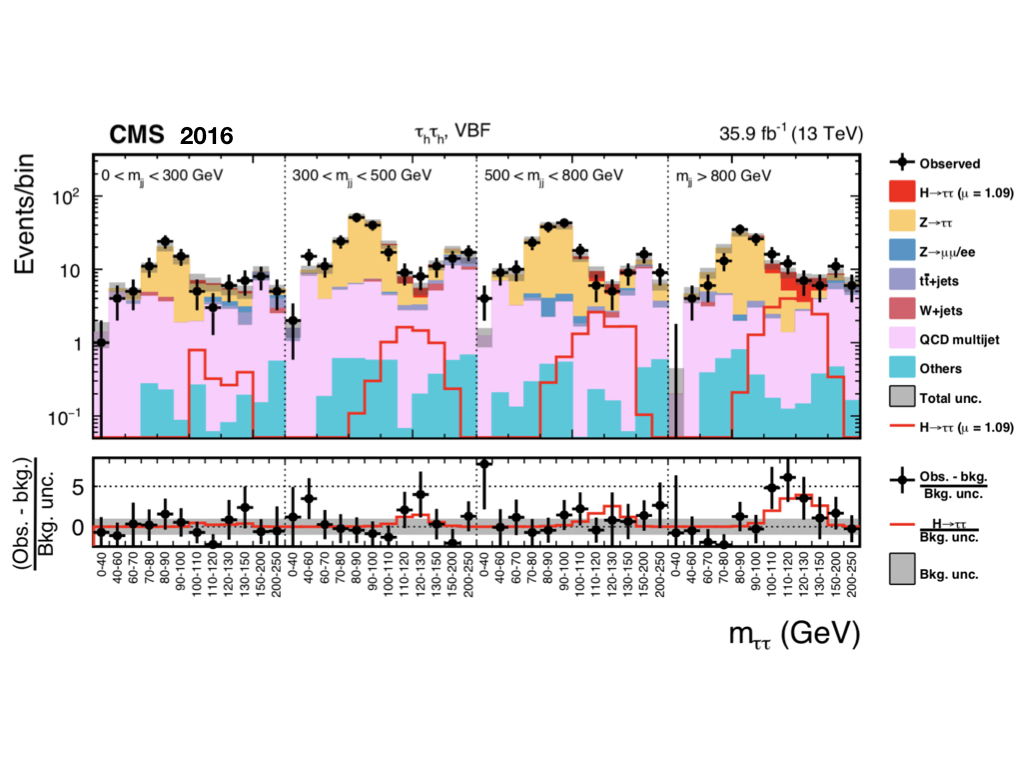
\includegraphics[trim=0 120 0 120,clip,width=0.75\textwidth]{HTT_Plots_2016.jpeg}
     \caption{Observed and predicted 2D distributions in the VBF category of the $\tau_{h}\tau_{h}$ channel from the public 2016 analysis. The bins are unrolled in $m_{jj}$ with slices corresponding to $m_{jj} = [0,350,500,800,+]$.}
     \label{fig:vbf_2016}
\end{figure*}

\begin{figure}[h]
\centering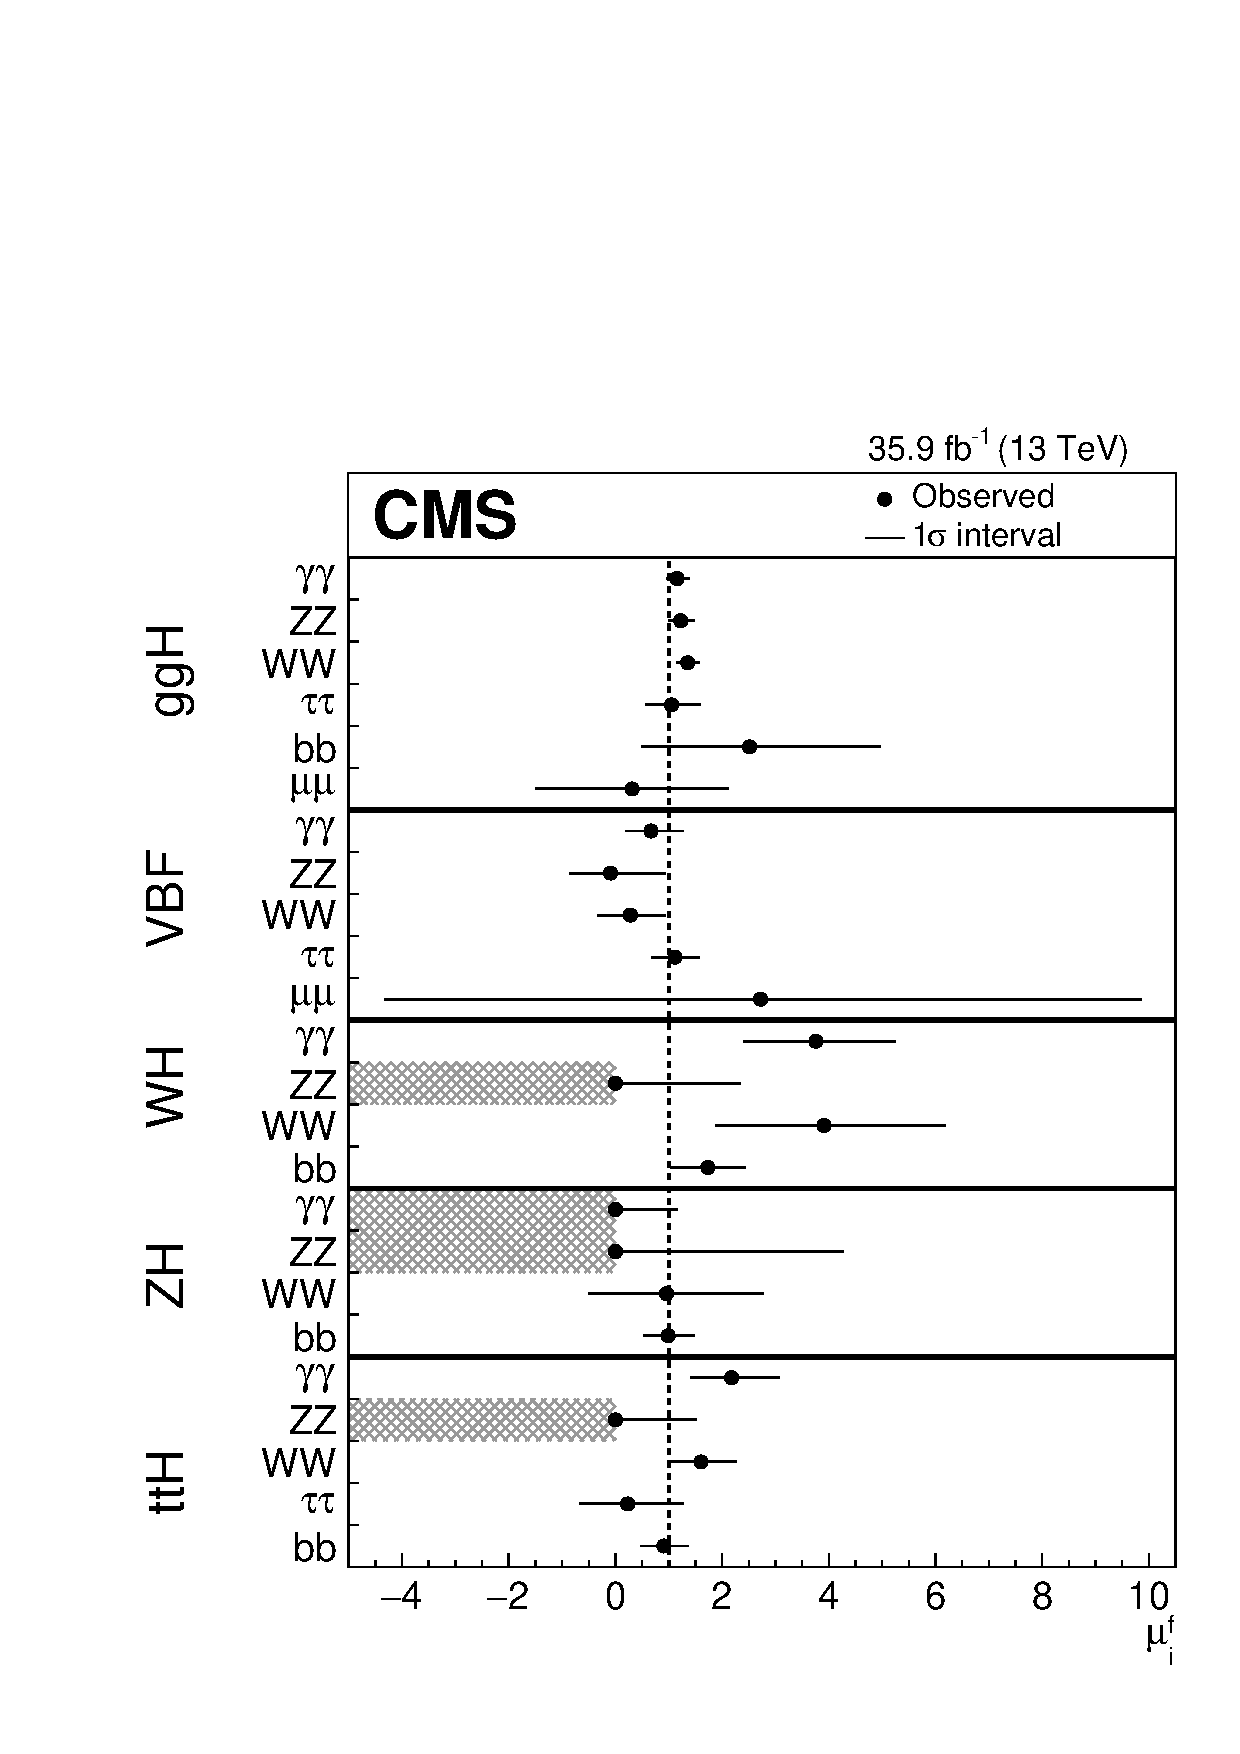
\includegraphics[width=0.4\linewidth]{CMS-HIG-17-031_Figure_006_VBF_Comparison.pdf}
\caption{In comparison with $\gamma\gamma$, ZZ, WW, bb and $\mu\mu$, the $\tau\tau$ final state provides the most stringent measurement of the VBF production mechanism~\cite{Sirunyan:2018koj} at CMS.}
\label{fig:Sirunyan2018koj}
\end{figure}

\subsection{Simplified Template Cross Section Measurement with the Run 2 Dataset}
Since Run 1, Simplified Template Cross Sections (STXS) have been adopted by the LHC 
experiments as a common framework to perform Higgs measurements. Their primary purpose 
is to reduce the theory 
dependencies that must be directly folded into Higgs precision measurements while at the same 
time allowing for the combination of the measurements between different decay channels as well 
as between experiments. In addition to using the $\tau\tau$ final state to measure the gluon
fusion and VBF production mechanisms, we are now measuring the Higgs as a function of the STXS,
consequently, the categories from 2016 have been redefined to better match the STXS binning.
The VBF category with low di-$\tau$ $p_{T}$ from the $\tau_{h}\tau_{h}$ channel corresponding
from the full Run 2 dataset can be seen in Fig.~\ref{fig:prefit_vbflow}.
I am the editor of this analysis and supervising one graduate student from Princeton,
one from Kansas State University and one from the University of Wisconsin-Madison.
I propose to continue leading this measurement until it is published and to extend
it to differential cross section measurements of the Higgs as a function
of the Higgs $p_{T}$ and as a function of the number of jets. 

\begin{figure*}[htbp]
\centering
     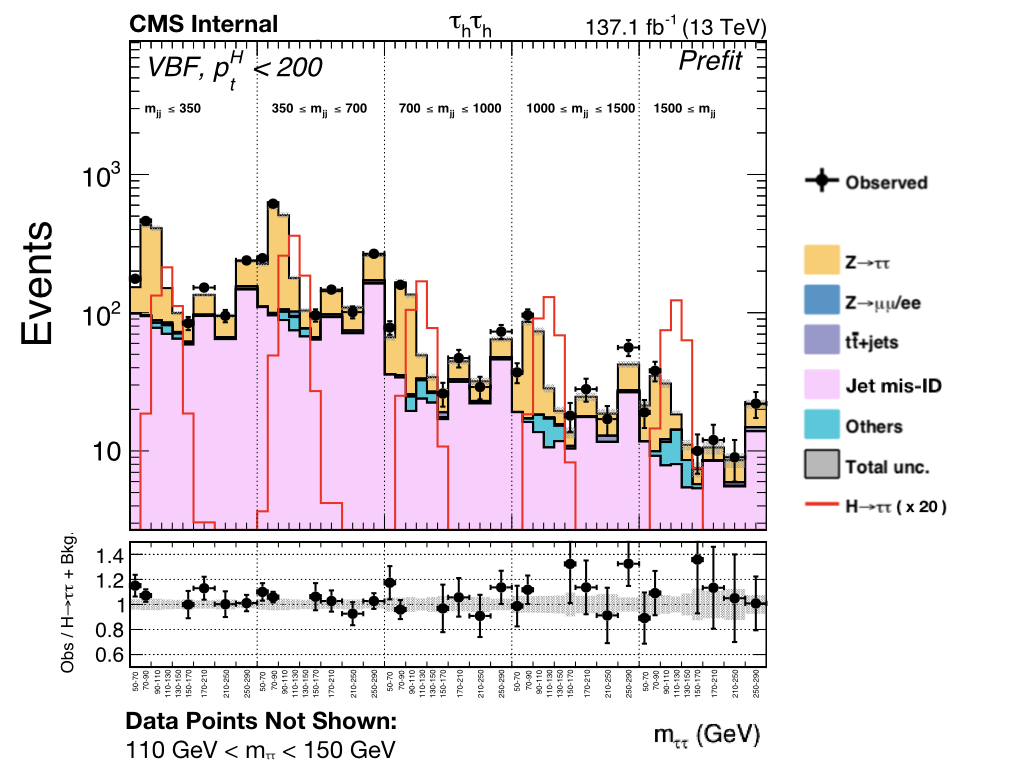
\includegraphics[width=0.65\textwidth]{HTT_Plots_combined.jpeg}
     \caption{Observed and predicted 2D distributions in the VBF category with low di-$\tau$ $p_{T}$ of the $\tau_{h}\tau_{h}$ channel. The bins are unrolled in $m_{jj}$ with slices corresponding to $m_{jj} = [350,700,1000,1500,+]$. \textbf{This analysis is currently being prepared for publication.} Bins with a high ratio of Higgs signal to SM background are blinded.}
     \label{fig:prefit_vbflow}
\end{figure*}

\subsection{MSSM Higgs $\rightarrow\tau\tau$}
The minimal supersymmetric standard model (MSSM) is one of the simplest extensions of the SM~\cite{FAYET1975104,FAYET1977489}.
The MSSM is a supersymmetric model invoking a symmetry between bosons and fermions,
which allows for a possible cancellation of the quadratically divergent self-energy 
corrections to the Higgs mass at high energy~\cite{WESS197439}.
At tree level, the Higgs sector of the MSSM can be expressed in terms of two free parameters. 
These are usually chosen to be the mass of the pseudoscalar Higgs boson, $m_{A}$, 
and the ratio of vacuum expectation values of the two doublets, tan~$\beta$. The dominant production mechanism in 
the MSSM is the gluon fusion process for small and medium values of tan~$\beta$. Large values of 
tan~$\beta$ indicate enhanced couplings to down-type fermions, resulting in b-associated production 
becoming dominant. Additionally the coupling to $\tau$ leptons is enhanced in this region, making 
searches in the di-$\tau$ final state excellent probes of the MSSM.
As a postdoc at the University of Wisconsin - Madison, I supervised two students on this analysis 
using the 2015 dataset  \cite{CMS-PAS-HIG-16-006}. Fig.~\ref{fig:mssm_2015} shows the expected and observed limits on cross-section 
times branching fraction for the gluon fusion and b-associated production processes resulting from the
combination of the channels $\tau_{\mu}\tau_{h}$, $\tau_{e}\tau_{h}$, $\tau_{h}\tau_{h}$, and $\tau_{e}\tau_{\mu}$.

\begin{figure*}[htbp]
\centering
     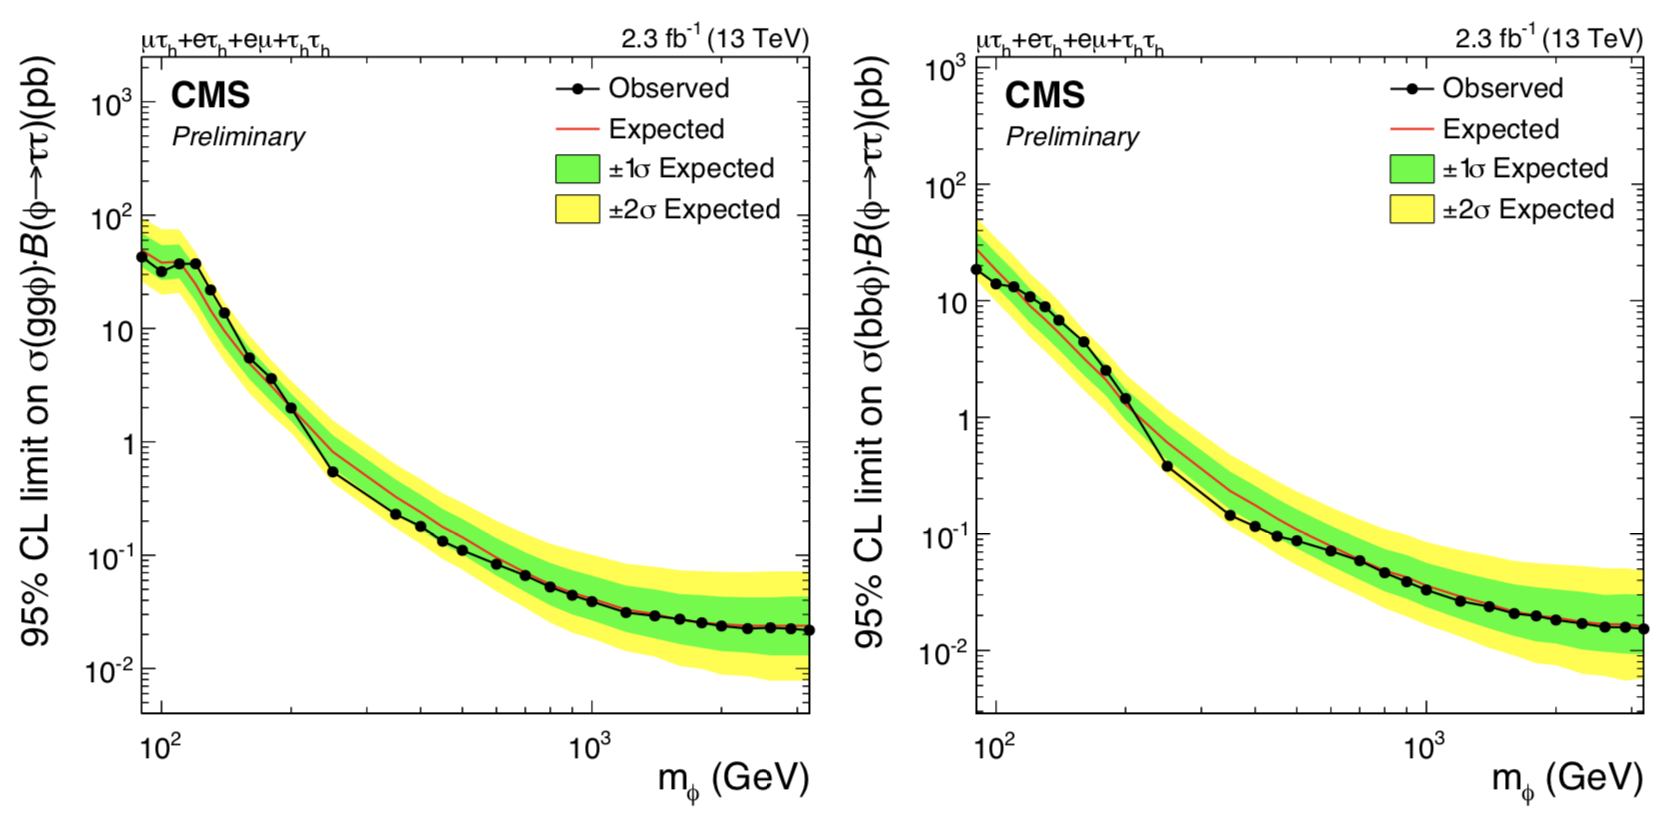
\includegraphics[width=0.9\textwidth]{limits-mssm.png}
     \caption{Expected and observed limits on cross-section
       times branching fraction for the gluon fusion and b-associated production processes resulting from the
       combination of the channels $\tau_{\mu}\tau_{h}$, $\tau_{e}\tau_{h}$, $\tau_{h}\tau_{h}$, $\tau_{e}\tau_{\mu}$. As a postdoc
     at the University of Wisconsin-Madison I supervised two students on this analysis.}
     \label{fig:mssm_2015}
\end{figure*}

After the SM $H\rightarrow\tau\tau$ Run 3 result is 
published my group, including postdoc Pallabi Das and graduate student Stephanie Kwan, will continue 
this search pursuing 
the three most sensitive channels: $\tau_{\mu}\tau_{h}$, $\tau_{e}\tau_{h}$, $\tau_{h}\tau_{h}$.
The 2015 and early 2016 results already extended the reach beyond that obtained in Run-1, however, much of the parameter space is 
still unexplored, and our efforts with the full Run-2 dataset will improve the discovery potential.

\section{CMS Level-1 Trigger Overview and Responsibilities}
The LHC is a two-ring superconducting hadron accelerator and collider with a designed center 
of mass energy of 14~TeV. For the original design luminosity of 10$^{34}$~cm$^{–2}$~s$^{-1}$,
25 inelastic collisions occur on average for every beam crossing with a frequency of 40~MHz.
This input rate of 10$^9$ interactions per second is reduced by a factor of 10$^6$ to 1 kHz,
the maximum rate that can be stored for offline analysis. 
The CMS trigger system is responsible for this online selection of events that are destined for full 
reconstruction and data analysis offline. The CMS trigger system comprises two levels~\cite{Khachatryan:2016bia}: 
The first level, Level-1 (L1), consists of custom hardware processors that receive data from the calorimeter and muon 
systems, generating a trigger signal within 3.5 microseconds, after which
no more than 100 kHz of the stored events are forwarded to the High Level Trigger (HLT). The L1 utilizes
custom electronics to identify, find the position of and sort in importance physics objects such as
electrons, muons, jets, and taus as well as the sum of missing energy. Upgrades to the LHC during Long Shutdown 1 (LS1)
resulted in an increase to the LHC design luminosity by 50\%, while the CMS L1 trigger rate
remained limited to 100~kHz by the readout electronics. This necessitated the Phase 1 upgrade 
to the L1 trigger,
which was successfully installed in two stages in 2014 and 2015 and fully operational for 
the 2016 run. For the
HL-LHC running, planned to start in 2026, the luminosity is to exceed 5x10$^{34}$~cm$^{–2}$~s$^{-1}$,
necessitating a complete overhaul of the CMS architecture to use tracking in the L1 for the first time
with a L1 rate up to 750~kHz, HLT rate up to 7.5~kHz and a completely new trigger system.

As a postdoc with the University of Wiscsonsin - Madison under the mentorship of Professors Wesley Smith
and Sridhara Dasu, I was responsible for the development and deployment of the online software for the 
Layer-1 of the calorimeter trigger system (2014-2016), calorimeter calibration (2016), installation of 
the $\mu$TCA electronics and development of the 2015 version of the Level-1 Tau Trigger for the 2015 and 2016 
upgrades. Currently I serve as the US CMS Operations deputy for the Level-1 trigger. My postdoc
Pallabi Das is participating in mid-week global runs at Point 5 (the CMS control room), graduate student
Stephanie Kwan will be moving to CERN in June and will also be participating in operations.

\subsection{Calorimeter Trigger and Phase-1 Upgrades}
%%%%Shorten me
During Run-1, the CMS Level-1 $e/\gamma$, $\tau$, jet, and missing transverse energy trigger decisions were based
on the processing of the Regional Calorimeter Trigger (RCT), which received input from the
CMS hadron calorimeter (HCAL) and electromagnetic calorimeter (ECAL), and the hadron calorimeter in
the very forward region (HF). The RCT forwarded the found $e/\gamma$, $\tau$, and jet candidates 
to the Global Calorimeter Trigger (GCT) for refining, sorting and transmission to the level-1 Global Trigger.
The upgraded ECAL provided an optical input path with duplicate information to the RCT and
Upgrade Calorimeter Trigger (UCT) so that both systems could be
operated in parallel with physics data during the transition period. 
Due to an upstream split, the upgraded HCAL electronics were operated in parallel with the original 
HCAL electronics, connected to the RCT and UCT, respectively.

The UCT successfully operated in parallel with the existing RCT system until it became the 
main calorimeter trigger in Sept. 2015 and provided for the first
time per-event pile-up subtraction in Level-1 triggers. 
Prof. Dasu and I developed the $\tau$ trigger algorithm for the UCT which used a reduction in feature size and experienced a 50\% increase in efficiency
to 95\% and a factor of 10 reduction in rate, as can be seen in Fig.~\ref{fig:tau_stage1}.
Using algorithms developed by groups from UW, Fermilab and MIT 
the performance in proton-proton running was considerably improved, the UCT also enabled an efficient trigger menu for 2015 Heavy Ion
running, which was not possible with the original trigger designed for lower HI luminosity.

\begin{figure*}[htbp]
    \centering
    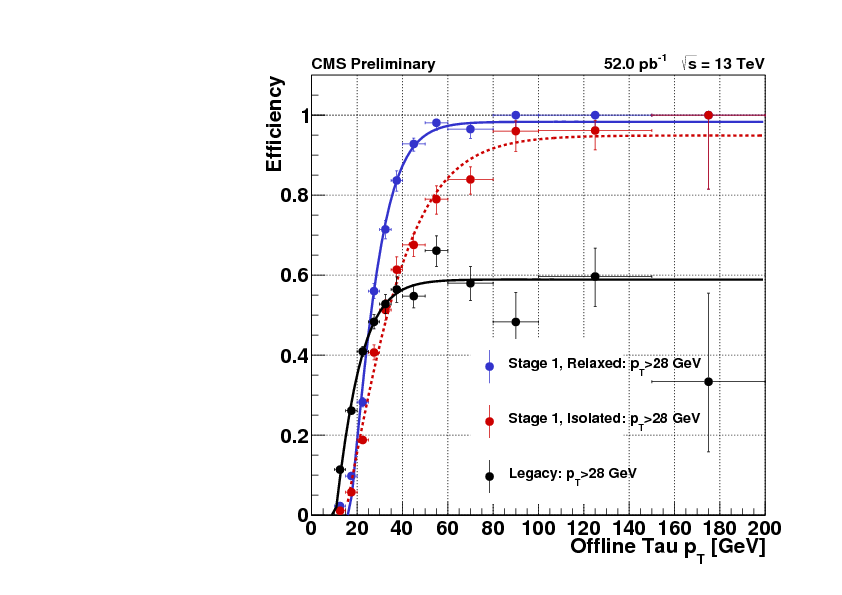
\includegraphics[trim=260 60 50 50,clip,width=0.45\textwidth]{TDR_RlxIsoLegacy_28GeV.png}
    \centering \caption{Isolated and relaxed (no isolation requirement) tau trigger efficiency as a 
       function of offline transverse momentum ($p_{T}$) for an online requirement of $p_{T}$) $\>$ 28 GeV. The
       Run 1, or legacy, efficiency for taus is shown for comparison. Note the legacy algorithm
       was seeded with the logical OR of a L1 di-tau requirement and L1 di-jet requirement to improve
       efficiency.}
     \label{fig:tau_stage1}
\end{figure*}

The Stage-2 UCT consists of 18 Calorimeter Trigger Processing cards which utilize a Xilinx Virtex-7 FPGA
as their primary processing device. They are distributed over 3 $\mu$TCA crates in layer-1. 10 MP7 cards 
(similar to the CTP7 built by the CMS-UK group) distributed over one
$\mu$TCA crate in layer-2 with an optical patch panel of up to 864 fibers in between. 
The system was run successfully in parallel system with the Stage-1 UCT starting in 
late 2015 and Stage-2 became the main calorimeter 
trigger in 2016. In addition, the Crosspoint I/O Cards (CIO) that provide bi-directional 
access to the Vadatech VT894 backplane as well
as backplane and inter-crate connections were installed. %The Stage-2 UCT system is shown in Figure 17. %% put in this figure

%%FIX ME%%
\subsection{Proposed Research Direction}
Since the luminosity is planned to increase, my group proposes to continue collaboration with the
University of Wisconsin (UW) group in development of new trigger algorithms using the Phase 1 trigger hardware in order to improve
physics signal capture during Run-3. The eighteen-CTP7 Layer-1 cards of UCT has over 60\% unused logic 
resources, enabling pre-computation of clusters as done in the RCT, in addition to continuing to serve 
UCT Stage-2 tower level data. We are focusing our efforts on three areas for improvement: Vector Boson Fusion  identification, Boosted Jet Substructure, and Long Lived Particle identification.
%% fix this 

\begin{figure}[h]
\centering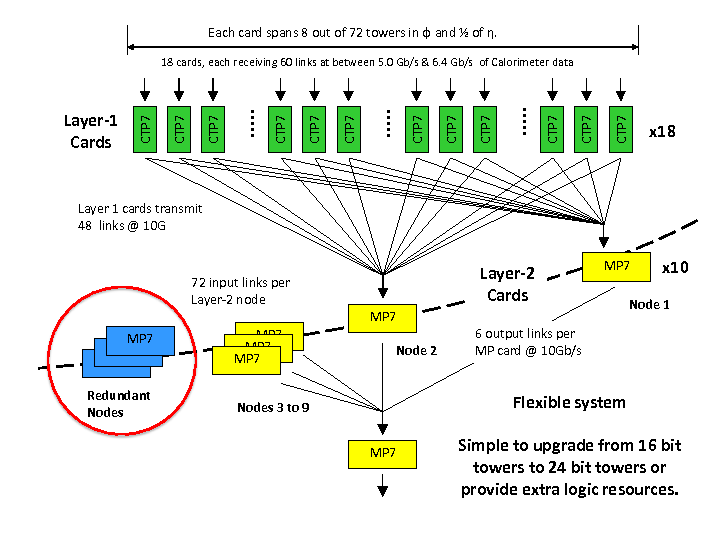
\includegraphics[width=0.5\linewidth]{stage2.png}
\caption{The Stage-2 UCT trigger system is shown. This trigger system was operated in parallel with the original UCT in 2015.
It acts as the primary calorimeter trigger system since 2016.}
\label{fig:CMS_L1_Trigger}
\end{figure}

\subsubsection{Vector Boson Fusion}
The very distinctive features of vector boson fusion production, with 
two jets back to back and along the direction of the beam line, presents
an excellent opportunity for distinguishing this Higgs production mechanism.
In offline analysis, tracks are used to reconstruct the primary collision vertex 
and jets which originate from this vertex are required to be back to back
in pseudorapidity and along the direction of the beam line. During trigger selection, 
the process of identifying jets which originate from the VBF process 
becomes more difficult as tracks are not available for vertex reconstruction.
In order to counter this we are developing a Deep Neural Network (DNN) based
identification that can be activated at the event-level. In order to combat
interference due to jets that originate from pile up, the DNN is trained 
using the four highest $p_{T}$ jets as well as event-level variables such
as the total $H_{T}$ of the event and an estimate of the Pile Up multiplicity
by counting the number of regions above a 1 GeV threshold.%does this need to be further explained?
%Initial estimates based on a VBF Higgs simulation sample and ZeroBias events
%taken from Run 3 show that this event-level trigger operates at 90% efficiency
%when atleast one jet above 40 GeV is present in the event for roughly a 1 kHz rate.

\subsubsection{Boosted Higgs}
Efforts to fully classify the nature of the Higgs are well underway at the LHC,
in addition to simply performing measurements as an effort to catalog a new 
and unique particle, any deviations from expectation could be due to underlying new physics
and motivate new searches or theoretical models. 
For instance, measurements of high-$p_{T}$ Higgs decays may resolve the loop induced 
and tree-level 
contributions to the ggF process~\cite{Grojean_2014} and provide an alternative 
approach to study the top quark Yukawa coupling in addition to the ttH process.
CMS recently published an inclusive search for a highly boosted Higgs boson decaying
to a bottom quark-antiquark pair~\cite{Sirunyan_HBB_2018}. 
In order to reconstruct the boosted Higgs candidate a single jet is clustered using
the anti-$k_{T}$ algorithm with a distance parameter of 0.8 (Ak8). This Ak8 jet is
then decomposed into sub-jets using the N$_{2}$ algorithm~\cite{Moult_2016}, 
which is based on a ratio of 2-point and 3-point generalized energy correlation 
functions (ECFs)~\cite{Larkoski_2013}, is exploited to determine how consistent a 
jet is with having a two-prong substructure.
The main experimental difficulties for this search originate from the large
cross section for background multi-jet events at low jet mass and the restrictive trigger requirements needed to reduce the data recording rate. 
At Level-1 the trigger requirement corresponds to a single high $p_{T}$ jet of at 
least 180~GeV which corresponds to an offline selection of 250~GeV. My group
is implementing a method to decompose jets at Level-1 into their two-prong 
sub-jet components.

The Level-1 trigger $\tau$ algorithm which was in place in 2015, used shape finding
to identify regions that are consistent with the topology of a hadronically
decaying $\tau$. In this algorithm, calorimeter towers in a 4 by 4 region are identified
as being "filled" if the tower contains at least 30\% of the energy in the 4 by 4 region.  
The region is then required to only contain filled tower configurations which are indicative
of a narrow energy deposit, as can be seen in Fig. \ref{fig_tau_algo}. Finally, in order
to account for possible overlap between neighboring regions, filled towers that pass shape
finding requirements and are on an edge are combined. %figure xxx
The result of implementing shape finding to identify hadronically
decaying $\tau$'s was an increase in efficiency from approximately 50\% to 95\%
and a reduction in rate by a factor of 3. 

We are implementing a similar methodology to identify AK8 jets with jet-substructure
online. Calorimeter towers in an 8 by 8 region are identified as being "filled" if the tower contains at least 10\% of the energy of the 8 by 8 region.  
The region is then required to only contain filled tower configurations which are indicative
of a two-prong jet structure. Examples of good shape are shown in Fig. %\ref{fig:}.%figure jet substructure

%\subsection{Long Lived Particle Identification}
%Particles beyond the Standard Model (SM) can generically have lifetimes that are long 
%compared to SM particles at the weak scale. When produced at experiments such as CMS, 
%these long-lived particles can decay far from the interaction vertex of the primary 
%proton-proton collision. Such LLP signatures are distinct from those of promptly 
%decaying particles that are targeted by the majority of searches for new physics 
%at the LHC, often requiring customized techniques for identification. 
%Future CMS upgrades destined for the HL-LHC will make use of these 

%The most sensitive method to search for $H\rightarrow bb$ decays at a hadron collider 
%is to use events in which the Higgs boson is produced in association with a W or Z boson 
%(VH) decaying to leptons, and recoiling with a large transverse momentum, in order to 
%suppress the overwhelming irreducible background from QCD multijet production of b quarks. 
%Because of this background, an observation of H(bb) decays in the gluon fusion 
%production mode was considered impossible. 

\subsection{Tau ID in the CMS Level-1 Trigger for the HL-LHC}
In its ultimate configuration, the HL-LHC will reach unprecedented performance in terms of instantaneous 
luminosity ($7-7.5 \times10^{34}$~$\mathrm{cm}^{-2}\mathrm{s}^{-1}$) 
leading to a total integrated luminosity of 4000 fb$^{-1}$ after ten years of
operations, which are scheduled to start in 2026.
This large increase in instantaneous luminosity necessitated a complete overhaul 
of the CMS architecture to use tracking in the Level-1 Trigger for the first time;
the upgraded L1 will have a latency of up to 13.5~$\mu$s and a maximum rate of 750kHz.

My group is working on designing the architecture and algorithms for the HL-LHC correlator 
trigger (CT) project. The CT system's purpose is
to correlate L1 tracks from the L1 track trigger with L1 calorimeter clusters from the
L1 calorimeter trigger and the high-granularity calorimeter and create L1 particle-flow objects (L1PF). 
This will be done in the first
layer (layer-1) of the correlator trigger. The second layer (layer-2) will be tasked with performing the 
reconstruction of high-level physics objects, namely, jets, $\tau$'s and Sums. Layer-2 will
also be tasked with the calculation of isolation quantities. 

I, along with my graduate student, Stephanie Kwan, have developed the first L1 Hadron-Plus-Strips (HPS).
This algorithm is firmly based on the offline HPS algorithm currently in use at CMS.
The offline $\tau$ candidates are formed by combining charged hadrons with photons that lie within 
narrow ECAL regions that extend in azimuth, also known as strips. Based on the observed number of 
strips and charged hadrons the $\tau$ candidate is assigned one of the following decay modes: 
a single charged hadron without any strips of photons: h$\pm$; a single charged hadron with one 
strip of photons: h$\pm\pi^{0}$; a combination of three charged hadrons: h$\pm$h$\mp$h$\pm$. 
The offline Hadron-plus-strips (HPS) algorithm uses the following input: charged hadrons, neutral 
hadrons, and photons reconstructed by the particle- flow algorithm. A version of the HPS algorithm 
suitable for the Level-1 Trigger, L1HPS, has been designed to use the above L1 PF input and 
is initiated by identifying at least one charged hadron above a seed $p_{T}$ threshold. Once a 
minimal charged-hadron seed is found, a search through nearby charged hadrons is initiated to: 
identify the candidate $\tau$ object as one- or three-prong, identify electron candidates that are 
later be used in $\pi^{0}$ finding, and determine isolation based on particle-flow candidates. 
The final stage of the L1HPS algorithm reconstruction determines an azimuthal strip containing possible photons 
from $\pi^{0}$ decays. 

After the $\tau$ candidate is reconstructed identification is performed using a Boosted Decision Tree (BDT)
which is used to distinguish true $\tau$'s from jets. The BDT was developed by Stephanie Kwan
and takes as input the position and $p_{T}$ of the $\tau$, the total isolation energy in a radius of $\Delta R$=0.4,
the $p_{T}$ and position of the strip and the position of the L1 primary vertex.
The performance of the L1HPS algorithm and the BDT can be seen in Fig.~\ref{fig:Phase_2_L1_Tau}.
The rate is calculated using a 200 pile-up sample and the efficiency is measured on a 200 pile-up
H$\rightarrow\tau\tau$ monte-carlo sample.

A prototype of the L1HPS tau algorithm was implemented in firmware using 
Vivado HLS on a testbench for a Virtex Ultra- scale+ (VU9P) FPGA with a 320 MHz clock. The HLS 
tool shows that the algorithm can process a new event once every bunch crossing with a latency 
of 20 bunch crossings, or approximately 0.5 $\mu$s. The required resource usage for this prototype 
algorithm to find 8 (4) tau candidates in an event is approximately 31\% (17\%) of FF and 42\% 
(21\%) of LUTs available on a Xilinx Ultrascale+ VU9P FPGA. 

\begin{figure}[h]
\centering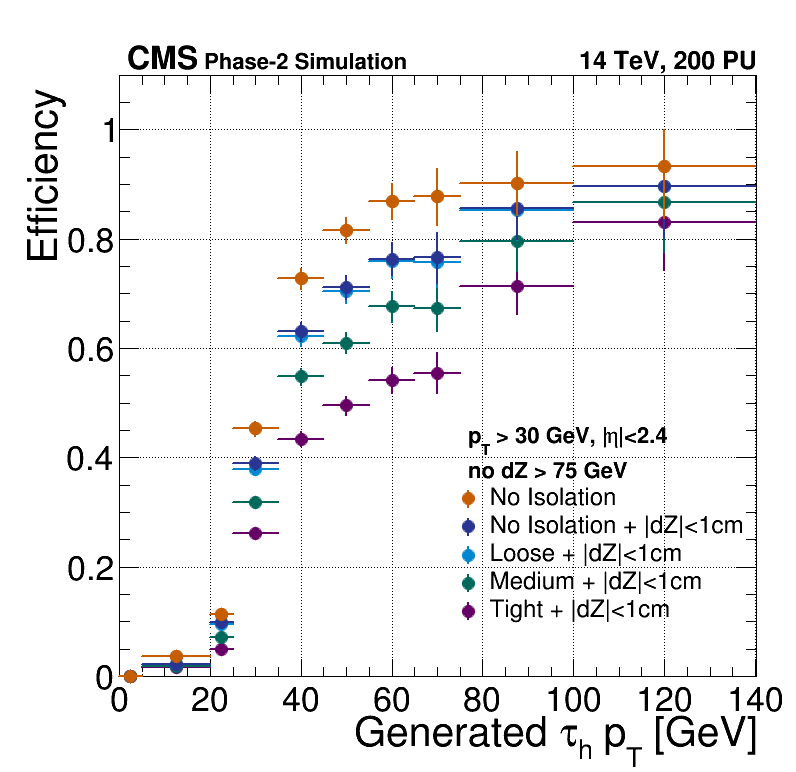
\includegraphics[width=0.45\linewidth]{genPt_1_DZ_2p4.png}
\centering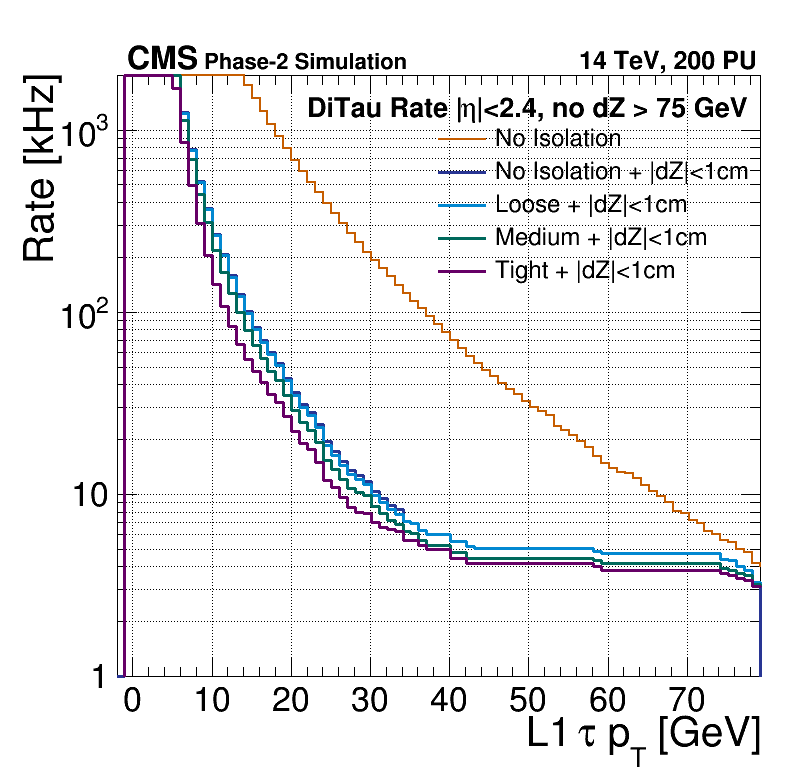
\includegraphics[width=0.45\linewidth]{l1DiTau_pt_eta2p4-thresh75.png}
\caption{Phase 2 Tau L1HPS algorithm performance with working points based on BDT from graduate student Stephanie Kwan}
\label{fig:Phase_2_L1_Tau}
\end{figure}

\subsection{Proposed Research Direction}
I propose to continue development of algorithms for the Phase~2 Level-1 correlator trigger system.
My group will participate in algorithm and architecture design. Based on this development 
hardware preproduction phase will advance the
prototype designs to incorporate all features and algorithms required for
production: preliminary choice of hardware FPGA and optical link speed,
a complete set of firmware algorithms, commonly compatible infrastructure
firmware, and required software for operation and performance testing.
After this is completed we will participate in vertical slice tests to
verify interface functionality and eventual installation and commissioning.

\section{Conclusions}
The next three years at the LHC will be an exciting time. 
The analysis of the full Run 2 dataset has begun; my group proposes to analyze this
dataset in the simplified template cross-section scheme to make precision measurements 
of the Higgs in its decay to $\tau$ leptons.
We will then extend this analysis to search for MSSM higgses by tagging events that are
produced in association with b flavor jets.

The LHC is currently in the middle of its second 
Long Shutdown and with this comes the opportunity to improve data taking for the LHC 
Run 3 and the HL-LHC. 
My group proposes to use this time to implement algorithmic advancements to the Level-1 
trigger in order to improve the current best measurements on VBF Higgs production and 
subsequent decay to $\tau$ lepton pairs in collaboration with the
group at the University of Wisconsin-Madison.


\newpage
%% The Appendices part is started with the command \appendix;
%% appendix sections are then done as normal sections
%% \appendix

%% \section{}
%% \label{}

%% References
%%
%% Following citation commands can be used in the body text:
%% Usage of \cite is as follows:
%%   \cite{key}          ==>>  [#]
%%   \cite[chap. 2]{key} ==>>  [#, chap. 2]
%%   \citet{key}         ==>>  Author [#]

%% References with bibTeX database:

%\bibliographystyle{model1-num-names}

%\bibliography{sample.bib}
\printbibliography

%% Authors are advised to submit their bibtex database files. They are
%% requested to list a bibtex style file in the manuscript if they do
%% not want to use model1-num-names.bst.

%% References without bibTeX database:

% \begin{thebibliography}{00}

%% \bibitem must have the following form:
%%   \bibitem{key}...
%%

% \bibitem{}

% \end{thebibliography}


\end{document}

%%
%% End of file `elsarticle-template-1-num.tex'.
